\documentclass{standalone}
\usepackage{tikz}
\usepackage{ctex,siunitx}
\setCJKmainfont{Noto Serif CJK SC}
\usepackage{tkz-euclide}
\usepackage{amsmath}
\usetikzlibrary{patterns, calc,3d}
\usetikzlibrary {decorations.pathmorphing,decorations.pathreplacing,decorations.shapes}
\begin{document}
\small
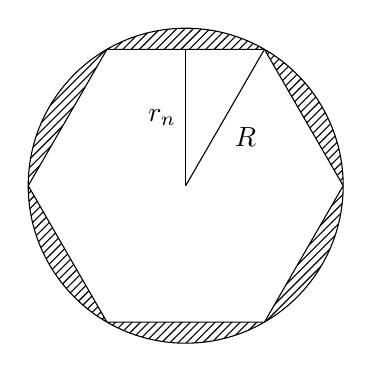
\begin{tikzpicture}[>=latex,scale=1.0]
  \draw[pattern=north east lines,even odd rule]
  (0,0)circle(2)
  (0:2)--(60:2)--(120:2)--(180:2)--(240:2)--(300:2)--cycle;
  \draw(0,0)--(60:2)node[midway,below right]{$R$};
  \draw(0,0)--(0,{sqrt(3)})node[midway,left]{$r_n$};
\end{tikzpicture}
\end{document}